\chapter{Helium Impurities and Interaction with Lithium}
\textit{This chapter has been submitted as journal article for peer review. The authors are A. Rafi M. Iasir and Karl D. Hammond of the University of Missouri.}

\section{Introduction}
Lithium is potentially an important element in the context of magnetic fusion
devices. Lithium-coated surfaces have been tested in several fusion devices
around the world~\cite{bell2009plasma, mirnov2003li, sanchez2009impact,
tuccillo2009overview, xu2011study, munaretto2012rfx} and have been found to
increase plasma confinement and improve plasma edge
conditions~\cite{allain2012lithium}.
This behavior is due in part to lithium's ability to trap hydrogen
isotopes~\cite{erents1971trapping}, which has the net result of decreasing
fuel recycling at the plasma edge, leading to higher confinement and fewer
disruptions~\cite{allain2012lithium}.
%Lithium reacts with hydrogen to form lithium hydride (LiH), which is
%ionic in nature.
Lithium has also been proposed as a tritium-breeding material in fusion
reactors~\cite{hartley1978potential} and as a liquid wall-coating ``armor''
to protect plasma-facing components~\cite{Kessel2019}.
%The recent interest in using solid lithium (applied to a graphite or
%tungsten surface) in fusion reactors is for density and impurity control in the
%temperature range of 30--50 \textdegree C~\cite{allain2012lithium}.
In the near-surface region of plasma-facing materials, high densities of
interstitials and vacancies are produced and high concentrations
of hydrogen and helium are present.
These defects and impurities will change the microstructure of the
material~\cite{Hammond2017c}.
It is therefore important to determine the energies of defects in lithium and
their interactions with helium.
This study calculates the energies of several point defects in lithium as
well as the formation, binding, and migration energies of helium atoms and
clusters trapped in lithium. 

\section{Methodology}
We performed all of our calculations using density functional theory (DFT) with
plane-wave basis sets as implemented in the software \textsc{QuantumESPRESSO}~\cite{giannozzi2009quantum}. Projector augmented wave
(PAW)~\cite{blochl1994projector} pseudopotentials from \textsc{QuantumESPRESSO}'s PS library~\cite{dal2014pseudopotentials,pp1} were used.
The density functional of Perdew, Burke, and Ernzerhof (PBE) was used as the
exchange--correlation functional~\cite{Perdew1996b, Perdew1997}. We used a
$4\times4\times4$ supercell of bcc lithium, which consists of 128 atoms, to
simulate defects. Brillouin zone sampling was performed using the scheme of
Monkhorst and Pack~\cite{monkhorst1976special} with a $k$-point mesh of
$5\times5\times5$. The plane wave cutoff energy was 50 Ry. The equilibrium
lattice parameter obtained was 3.436 \AA\@ for bcc lithium. All defect
calculations were performed by fully relaxing the atomic positions in the
supercell at constant volume using this lattice parameter.
The migration energies were calculated using the
nudged elastic band method~\cite{Jonsson1998, henkelman2000climbing,
    henkelman2000improved}
with seven images along the migration pathway.

The formation energies are calculated as follows:
\begin{subequations}
\begin{gather}
 E_{f}^{\text{oct}}  = E_{\text{Li}+\text{He}_{\text{oct}}} - E_{\text{Li}_N} - E_{\text{He}_{\text{isolated}}} \\
 E_{f}^{\text{tetr}} = E_{\text{Li}+\text{He}_{\text{tetr}}} - E_{\text{Li}_N} - E_{\text{He}_{\text{isolated}}} \\
 E_f^{\Box} = E_{\text{Li}_{N-1}} - \frac{N-1}{N} E_{\text{Li}_N} \\
 E_f^{\text{subs}} = E_{\text{Li}+\text{He}_{\Box}} - \frac{N-1}{N} E_{\text{Li}_N} - E_{\text{He}_{\text{isolated}}}.
\end{gather}
 \end{subequations}
Here, $E_{\text{Li}+\text{He}_{\text{tetr/oct}}}$ is the energy of a system in
which helium is situated at either octahedral or tetrahedral sites in bcc
lithium. $E_{\text{Li}+\text{He}_{\Box}}$ is the energy of a system in which
helium is in a substitutional position, $E_{\text{Li}_N}$ is the energy of a
defect-free lithium supercell containing $N$ atoms, and
$E_{\text{He}_{\text{isolated}}}$ is the energy of an isolated helium atom.
$E_{\text{Li}_{N-1}}$ is the energy of a lithium bcc supercell with a lithium
self-vacancy present.

The formation energy of a self-interstitial atom (SIA) is calculated using
\begin{equation}
E_f^{\text{SIA}} = E_{\text{Li}_{N+1}} - \frac{N+1}{N} E_{\text{Li}_N},
\end{equation}
where $E_{\text{Li}_{N+1}}$ is the energy of a system with a lithium
self-interstitial atom starting in either an octahedral or tetrahedral
position. The binding energy of two helium atoms is determined via the formula
\begin{equation}
E_b^{\text{He}_1\text{--}\text{He}_2}
    = E_{\text{Li}_{N}+\text{He}_1} + E_{\text{Li}_{N}+\text{He}_2}
        - E_{\text{Li}_N+\text{He}_1 + \text{He}_2} - E_{\text{Li}_N}.
\end{equation}
Here, $E_{\text{Li}+\text{He}_1}$ is the energy of the supercell with a
single helium interstitial present, and
$E_{\text{Li}_N+\text{He}_1 + \text{He}_2}$
is the energy of the supercell containing two nearby helium atoms in
interstitial positions. For more than two helium atoms, the following equation
is used to calculate the binding energies between them:
\begin{equation}
E_b^{\text{He}_n} = \left (\sum_{i=1}^n E_{\text{Li}_N+\text{He}_i} \right ) - \left[ E_{\text{Li}_N+\text{He}_n} + (n-1)E_{\text{Li}_N} \right].
\end{equation}
The helium--helium dumbbell formation energy (two helium atoms sharing a vacancy) can be calculated using the following equation:
\begin{equation}\label{eq_hedmbl}
  E_f^{\text{He}-\Box-\text{He}}
  = E_{\text{Li}_{N-1}+\text{He}-\Box-\text{He}}
    - \frac{N-1}{N} E_{\text{Li}_N} - E_{\text{He}_{\text{isolated}}}.
\end{equation}
Here, $E_{\text{Li}_{N-1}+\text{He}-\Box-\text{He}}$ is the energy of a supercell containing the helium dumbbell.

\section{Results and Discussion}
We calculated the formation energies for different configurations of the
self-interstitial atoms and the vacancy formation energy for lithium. The
results are presented in Table~\ref{tab:lidmble}. Our results are comparable
with previous DFT calculations and with experiments. Earlier DFT studies
produced formation energies of lithium self-vacancies from 0.52 to
0.57~eV~\cite{benedek1992formation, Pawellek_1991, frank1993properties,
frank1996first}, compared to our value of 0.496~eV\@. The discrepancy could
come from the size of the supercell, elastic interaction, the density
functional, and the quality of the pseudopotential.

We also calculated the self-interstitial formation energy of lithium.
Octahedral self-interstitials are unstable and relax to a dumbbell oriented in
one of the \hkl<100> directions (Fig.~\ref{fig:dmbl}). Tetrahedral
self-interstitials are also unstable and relax to \hkl<110> dumbbells. The
lowest-energy dumbbell orientations are the \hkl<111> orientations, which is a
similar trend as in other non-ferromagnetic bcc materials. The vacancy
formation energy is slightly lower than Frank \etal's value
(0.52~eV)~\cite{frank1996first} and Ma and Dudarev's value
(0.506~eV)~\cite{ma2019effect}, while the migration energy of the vacancy in
\hkl<111> directions is slightly higher than that found by Ma and
Dudarev~\cite{ma2019effect}.
The self-interstitial dumbbell formation energy is comparable to the values
reported by Ma and Dudarev~\cite{ma2019}.

\begin{figure}
	\centering
	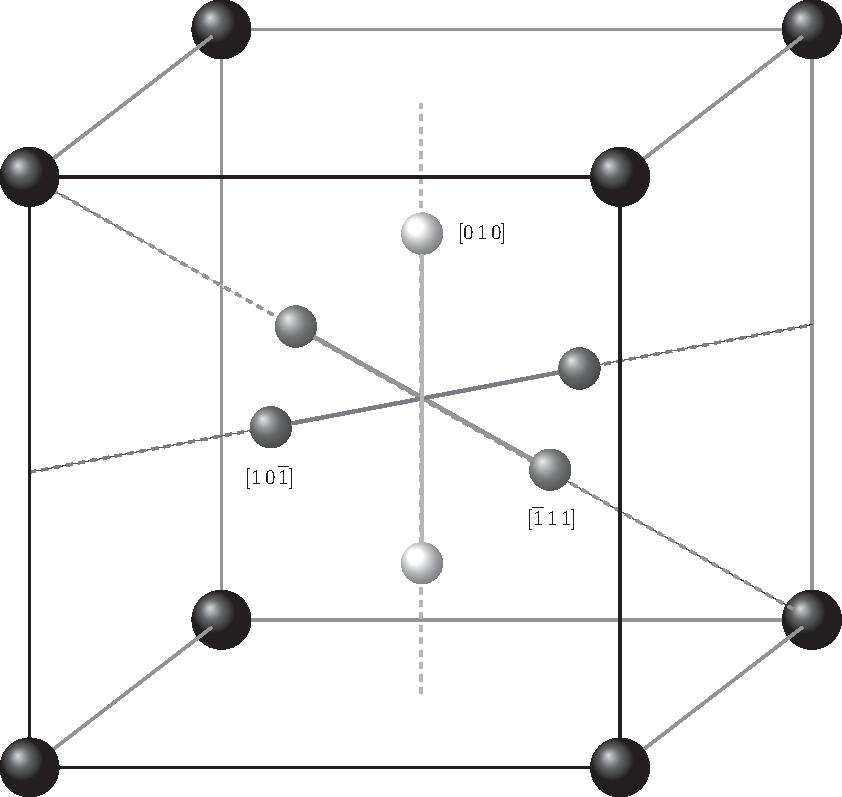
\includegraphics[width=3.3 in]{bcc-dumbbells}
	\caption{Helium--helium dumbbells in different orientations in the bcc
        lithium unit cell.}
	\label{fig:dmbl}
\end{figure}

\begin{table}
\caption[Calculated vacancy formation energy $E_f^{\Box}$, vacancy migration
    energy $E_m^\Box$, and various split-dumbbell and self-interstitial
    formation energies in lithium]{Calculated vacancy formation energy $E_f^{\Box}$, vacancy migration
    energy $E_m^\Box$, and various split-dumbbell and self-interstitial
    formation energies in lithium.
    Results are compared with previous theoretical and experimental results
    (experiments in italics).}
\label{tab:lidmble}
\centering
\renewcommand{\arraystretch}{1.2}
\begin{tabular}{l l l}
  \toprule
  Defect & Energy (eV) & Previous Work \\
  \midrule
  vacancy ($E_f^{\Box}$)
    & 0.496 & 0.506~\cite{ma2019effect} \\
    & & 0.52~\cite{frank1996first} \\
    & & \textit{0.508}~\cite{LandoltBornstein1991} \\
  vacancy ($E_m^\Box$) & 0.086 & 0.053~\cite{ma2019effect} \\ 
    & & \textit{0.038}~\cite{LandoltBornstein1991} \\ 
  \hkl<111> dumbbell ($E_f$) & 0.589 & 0.573~\cite{ma2019} \\
  \hkl<110> dumbbell ($E_f$) & 0.646 & 0.637~\cite{ma2019} \\
  \hkl<100> dumbbell ($E_f$) & 0.791 & 0.782~\cite{ma2019} \\
  tetrahedral ($E_f^{\text{tetr}}$)$^a$ & 0.646 & 0.696~\cite{ma2019} \\
  octahedral ($E_f^{\text{oct}}$)$^b$ & 0.793	& 0.785~\cite{ma2019} \\
  \bottomrule
  \multicolumn{3}{l}{$^a$ equivalent to \hkl<110> dumbbell formation} \\
  \multicolumn{3}{l}{$^b$ equivalent to \hkl<100> dumbbell formation} \\
\end{tabular}
\end{table}


\begin{table}
\caption[Formation energies ($E_f$), binding energies ($E_b$), and migration
  energies ($E_m$, all in eV)
  for helium located at octahedral or tetrahedral interstitial
  sites as well as substitutional sites]{Formation energies ($E_f$), binding energies ($E_b$), and migration
  energies ($E_m$, all in eV)
  for helium located at octahedral or tetrahedral interstitial
  sites as well as substitutional sites. The results are compared with helium
  interactions with tungsten and iron, which are both bcc metals at standard
  temperature and pressure.}
\label{tab:he_li} 
\centering
\renewcommand{\arraystretch}{1.45}
%\begin{minipage}{20.0em}
%\let\footnoterule\relax
\begin{tabular}{l l l l} \toprule
Quantity & Li--He & W--He~\cite{Becquart2006}
    & Fe--He~\cite{seletskaia2005magnetic} \\ \midrule
$E_{f}^{\text{oct}}$        & 1.142 & 6.38 & 4.60 \\
$E_{f}^{\text{tetr}}$       & 1.132 & 6.16 & 4.37 \\
$E_f^{\text{subs}}$         & 1.213 & 4.70 & 4.08 \\
$E^{\ce{T-T}}_m$            & 0.003 & 0.06 & 0.06 \\
$E^{\ce{T-O-T}}_{m}$        & 0.013 & & \\
$E^{\ce{O-O}}_{m}$          & 0.004 & & \\
${E^{\ce{He}-\ce{He}}_b}^a$ & 0.209	& 1.03 & \\ 
${E_b^{\ce{He_s-\Box}}}^b$      & 0.211 \\
${E_b^{\ce{He_t-\Box}}}^c$      & 0.421 \\
	\bottomrule
\multicolumn{4}{p{9 cm}}{$^a$both helium at nearest tetrahedral positions} \\
\multicolumn{4}{p{9 cm}}{$^b$one helium at a substitutional position interacting with
    a vacancy} \\
\multicolumn{4}{p{9 cm}}{$^c$one helium at a tetrahedral position interacting with a
    vacancy} \\
\end{tabular}
%\end{minipage}
\end{table}

\begin{table}
  \caption{Formation energies ($E_f$) of He--He split dumbbells bound to a
    vacancy.}
  \label{tab:hedmble}
  \centering
\renewcommand{\arraystretch}{1.2}
  \begin{tabular}{l l} \toprule
    Orientation & $E_f$ (eV) \\ \midrule
    \hkl<111>   & 1.844 \\
    \hkl<110>   & 1.863  \\
    \hkl<100>   & 1.879 \\ 
  \bottomrule
  \end{tabular}
\end{table}

We now turn our attention to helium interactions with lithium.
During the operation of a plasma device in which lithium is present,
any lithium-coated surfaces will interact with high fluxes of helium and
hydrogen isotopes.
There will also be (n,$\alphaup$) reactions that transmute lithium to
hydrogen and helium. These processes will build up a substantial amount
of hydrogen and helium inside the plasma-facing material. Significant research
has been and is still being performed to understand the behavior of helium in
metals~\cite{Hammond2017c,hammond2020theoretical, samaras2009}. 

One of the major challenges is the low solubility of helium in metals. Helium
atoms in a metal may find low-energy positions either in substitutional or
interstitial lattice sites. We calculated the formation energies of different
configurations of helium in substitutional as well as interstitial positions
in lithium.
The results are presented in Table~\ref{tab:he_li}. We compare our results to
similar configurations in tungsten and iron, two common bcc metals used in
plasma devices. Our calculations predict that the
tetrahedral interstitial position is the lowest-energy interstitial site for
helium, which is also the case for other bcc metals such as tungsten and
iron~\cite{Becquart2006,fu2005}. However, the difference between the octahedral
and tetrahedral interstitial formation energies is only 0.01~eV\@.
This is very low compared to tungsten--helium (0.22~eV~\cite{Becquart2006})
and iron--helium (0.23~eV~\cite{seletskaia2005magnetic})\@.

The formation energy of helium in a substitutional position in lithium is
1.213~eV, which is higher than both the tetrahedral and the octahedral
interstitial formation energies (which are 1.132~eV and 1.142~eV,
respectively).
This is an atypical result compared to helium in other bcc metals or
in fcc metals, for which the substitutional site has a significantly lower
formation energy than the two interstitial
sites~\cite{Becquart2006,seletskaia2005magnetic,Seletskaia2008,Liao2020},
and is more consistent with the energetics of helium in hexagonal close-packed
(hcp) metals~\cite{Yang2011a,Yang2011b}. 
We reproduced this result using a different DFT package
(\ie, \textsc{Abinit}~\cite{Gonze2020,Romero2020})
and got the same values. We also got similar values using ultrasoft
pseudopotentials in \textsc{QuantumESPRESSO}\@.
This is an intriguing result, and will have implications for future simulations
of helium in lithium.

\begin{figure}
	\centering
  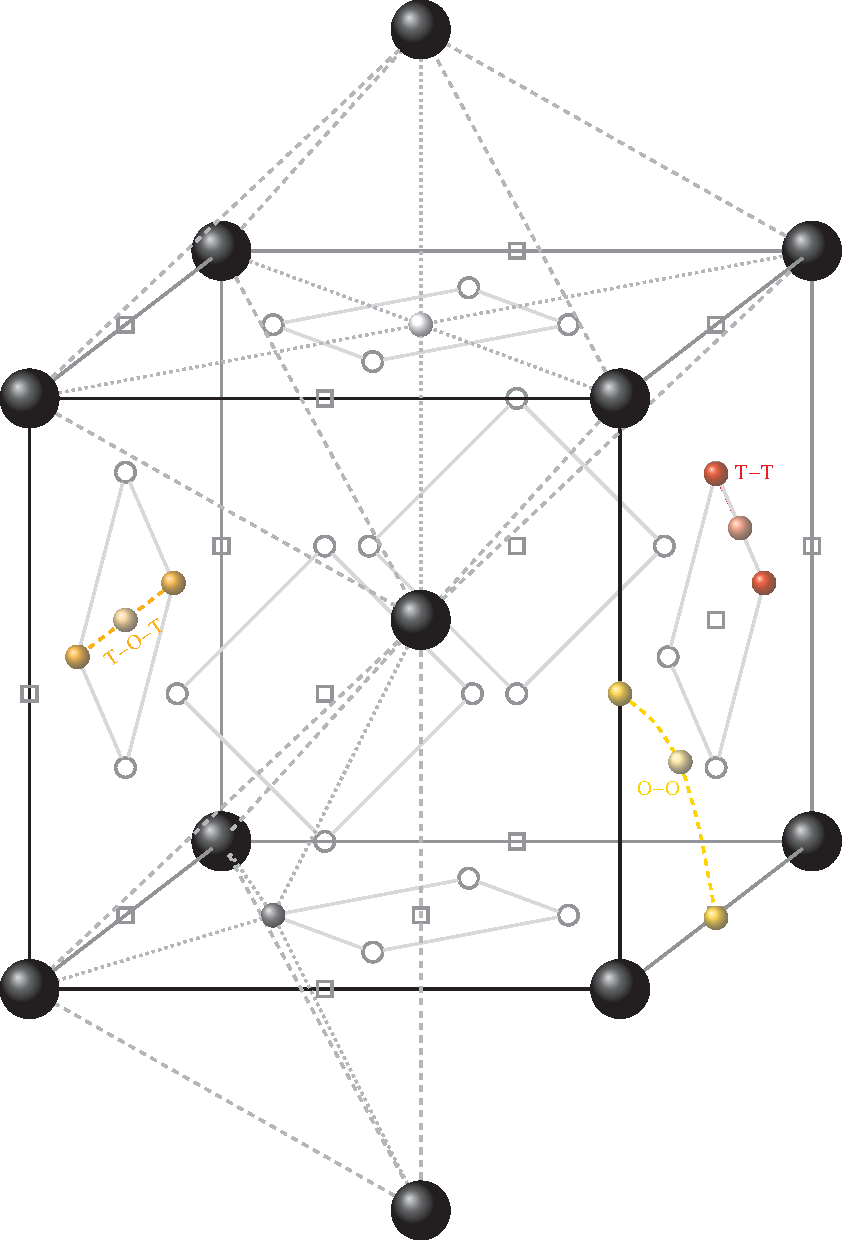
\includegraphics[width=3.9 in]{bcc-sites}
  \caption[Tetrahedral ({\scriptsize$\bigcirc$}) and octahedral ($\square$)
    sites in a bcc crystal]{Tetrahedral ({\scriptsize$\bigcirc$}) and octahedral ($\square$)
    sites in a bcc crystal.
    Three different transition states---tetrahedral to tetrahedral
    (\ce{T-T}), octahedral to octahedral (\ce{O-O}) and tetrahedral to
    octahedral to tetrahedral (\ce{T-O-T})---are shown.}
  \label{fig:tetr}
\end{figure}


Next, we calculated the binding energy of helium to a vacancy.
The substitutional formation energy is higher than the two interstitial
formation energies, though the substitutional site is still the energetic
minimum in the presence of a vacancy.
The binding energy of helium in a substitutional position to a vacancy is
0.21~eV\@.
The binding energy of helium at a tetrahedral interstitial site to a
vacancy is 0.42~eV\@.
The binding energy between two helium atoms at nearby interstitial sites is
0.209~eV, which is lower than that in the tungsten--helium system
(1.03~eV~\cite{Becquart2006}).
The binding energy of multiple helium atoms to a vacancy is also calculated,
and the result is shown in Fig.~\ref{fig:he-bind}. There is a nearly linear
increase in the binding energy as the number of helium atoms increases, which
indicates that a group of helium atoms will tend to aggregate onto a vacancy
and that helium bubble self-nucleation will likely occur in lithium, as it
does in other bcc metals~\cite{Sefta2013b}.


\begin{table}%[htbp]
  \caption{Binding energy of $n$ helium atoms to a vacancy.}
  \centering
  \begin{tabular}{l l}
  \toprule
    $n$ & $E_b$ \\
  \midrule
    %1 & 0.41544262703907636 \\
    %2 & 0.8976585425702422 \\
    %3 & 1.2488173959857483 \\
    %4 & 1.9027688203369273 \\
    %5 & 2.1936052126932073 \\
    %6 & 3.062218788587429 \\
    %7 & 3.2156586866844217 \\
    %8 & 3.9251163930455113 \\
    1 & 0.415\\
    2 & 0.898\\
    3 & 1.249\\
    4 & 1.903\\
    5 & 2.194\\
    6 & 3.062\\
    7 & 3.216\\
    8 & 3.925\\
  \bottomrule
  \end{tabular}
\end{table}


\begin{figure}
  \centering
  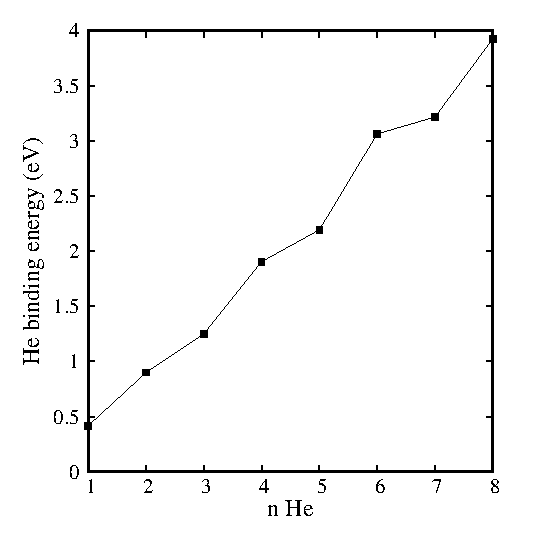
\includegraphics[width=3.8 in]{he-vac-bind-E}
  \caption{Binding energy of $n$ helium atoms to a vacancy for $n \in [1,8]$.}
  \label{fig:he-bind}
\end{figure}

Two helium atoms around a vacancy form a split dumbbell, much like lithium
self-interstitials do. The formation energy varies based on the orientation of
the dumbbell. The helium dumbbell formation energies are presented in
Table~\ref{tab:hedmble}.
The lowest-energy dumbbells have \hkl<111> orientations~(Fig.~\ref{fig:dmbl}).

The migration energies of helium from one tetrahedral site to a nearby tetrahedral site (Fig.~\ref{fig:tetr}) were calculated using the nudged elastic band
method~\cite{Jonsson1998, henkelman2000climbing, henkelman2000improved}.
The migration energy from one tetrahedral site to an adjacent tetrahedral site
(Fig.~\ref{fig:tetr}) is only 0.003~eV, indicating that helium interstitials
will be very mobile in lithium. Helium has a higher migration energy
($E_{m}^{\ce{T-T}}$) in tungsten (0.06~eV~\cite{Becquart2006}) and
iron (0.06~eV~\cite{fu2005}).
The migration energy from one octahedral site to the next octahedral
site ($E_{m}^{\ce{O-O}}$) without passing through a tetrahedral site in lithium
is 0.004~eV, which is also very low.
The low migration energies indicate that helium would be highly mobile in bulk
lithium, much more so than in other bcc metals. It also indicates that bulk
helium diffusion in lithium would be more akin to diffusion in gases or
liquids, with a $T^{3/2}$ dependence of the diffusion coefficient arising from
translational motion, but without the Arrhenius temperature dependence
associated with vibrational motion. This result, combined with the higher
formation energy of substitutional helium compared to interstitial helium,
suggests that helium transport in lithium will be fundamentally different than
it is in iron, nickel, tungsten, and other metals.

\nomenclature{$E_f^{\text{subs}}$}{helium formation energy in a substitutional position}
\nomenclature{$E_f^{\text{tetr}}$}{helium formation energy in a tetrahedral position}
\nomenclature{$E_f^{\text{oct}}$}{helium formation energy in a octahedral position}
\nomenclature{$E_{\text{He}_{\text{isolated}}}$}{energy of an isolated helium atom}
\nomenclature{$E_f^{\text{He}-\Box-\text{He}}$}{helium--helium dumbbell formation energy around a vacancy}
\nomenclature{$E_b$}{binding energy}

\clearpage
\bibliographystyle{apsrev4-2}
\bibliography{abbreviated,final}

